\section{Object Design}
In questa fase si descrivono gli oggetti facenti parte del sistema e le componenti di terze parti utilizzate per la realizzazione del progetto.
\subsection{Componenti di Terze Parti}
PocketDev fa uso di varie librerie e tecnologie per la sua realizzazione:
\begin{itemize}
 \item Javascript: Linguaggio interpretato di scripting utilizzato per la realizzazione della logica di business e della pagina principale;
 \item HTML, CSS: Tencologie Web di base per la realizzazione di contenuti;
 \item KnockoutJS: Libreria per la realizzazione di interfacce dinamiche javascript tramite il pattern MVVM (Model-View-ViewModel);
 \item NodeJS: Ambiente per eseguire codice javascript al di fuori del browser; Presenta un' architettura di tipo Event-Driven ottima per gestire grossi carichi di lavoro;
 \item ExpressJS: libreria Javascript per Node utile per creare servizi REST in maniera semplice;
 \item Apache Fuseki: Funge da servizio per interrogare il database tramite SPARQL e serializzare il risultato in un formato compatibile per il web.
 \item TDB: Database che memorizze in formato efficiente triple in RDF;
 \item RDF: Sta per resource description framework e serve per descrivere la base di dati semantica tramite triplette di concetti;
 \item SPARQL: linguaggio per effettuare interrogazioni sul database semantico;
 \item Protégé: Ide grafico per la realizzazione dell'ontologia ideato dalla Stanford university;
\end{itemize}
\subsection{Diagramma delle classi}
\begin{figure}[H]
 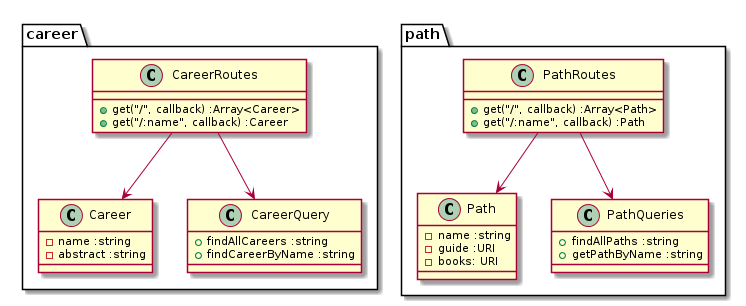
\includegraphics[scale=.5]{classdiagram.png}
\end{figure}
\subsection{Sviluppi Futuri}
Espandere l'ontologia può sicuramente arricchire la piattaforma con informaioni sempre più dettagliate e possibilmente eliminare lo scraper per avere una base di dati puramente semantica. 
